% Created 2020-06-08 lun. 11:40
% Intended LaTeX compiler: pdflatex
\documentclass{ISMA_USD2020}
\usepackage[utf8]{inputenc}
\usepackage[T1]{fontenc}
\usepackage{graphicx}
\usepackage{grffile}
\usepackage{longtable}
\usepackage{wrapfig}
\usepackage{rotating}
\usepackage[normalem]{ulem}
\usepackage{amsmath}
\usepackage{textcomp}
\usepackage{amssymb}
\usepackage{capt-of}
\usepackage{hyperref}
\usepackage[most]{tcolorbox}
\usepackage{bm}
\usepackage{booktabs}
\usepackage{tabularx}
\usepackage{array}
\usepackage{siunitx}
\usepackage{amsmath,amssymb,amsfonts, cases}
\usepackage{algorithmic, graphicx, textcomp}
\usepackage{xcolor, import, hyperref}
\usepackage[USenglish, english]{babel}
\setcounter{footnote}{1}
\input{config.tex}
\author[1,3] {T. Dehaeze}
\author[1,2] {C. Collette}
\affil[1] {Precision Mechatronics Laboratory\NewLineAffil University of Liege, Belgium \NewAffil}
\affil[2] {BEAMS Department\NewLineAffil Free University of Brussels, Belgium \NewAffil}
\affil[3] {European Synchrotron Radiation Facility \NewLineAffil Grenoble, France e-mail: \textbf{thomas.dehaeze@esrf.fr}}
\date{}
\title{Vibration control of a rotating Stewart platform}
\hypersetup{
 pdfauthor={},
 pdftitle={Vibration control of a rotating Stewart platform},
 pdfkeywords={},
 pdfsubject={},
 pdfcreator={Emacs 27.0.91 (Org mode 9.4)}, 
 pdflang={English}}
\begin{document}

\maketitle

\abstract{
    Abstract text to be done
}

\section{Introduction}
\label{sec:org335669b}
\label{sec:introduction}


\section{Theory}
\label{sec:org8b756e7}
\label{sec:theory}

\subsection{Rotating Positioning Stage}
\label{sec:orgbf4a596}

\begin{figure}[htbp]
\centering
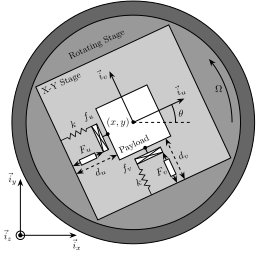
\includegraphics[scale=1]{figs/rotating_xy_platform.pdf}
\caption{\label{fig:rotating_xy_platform}Figure caption}
\end{figure}


\subsection{Equation of Motion}
\label{sec:orgaa8880a}

Let's express the kinetic energy \(T\) and the potential energy \(V\) of the mass \(m\):
\begin{align}
\label{eq:energy_inertial_frame}
T & = \frac{1}{2} m \left( \dot{x}^2 + \dot{y}^2 \right) \\
V & = \frac{1}{2} k \left( x^2 + y^2 \right)
\end{align}

The Lagrangian is the kinetic energy minus the potential energy.
\begin{equation}
\label{eq:lagrangian_inertial_frame}
L = T-V = \frac{1}{2} m \left( \dot{x}^2 + \dot{y}^2 \right) - \frac{1}{2} k \left( x^2 + y^2 \right)
\end{equation}


\subsection{Integral Force Feedback}
\label{sec:org754b644}


\subsection{Direct Velocity Feedback}
\label{sec:org9cbf82a}


\section{Conclusion}
\label{sec:org8d24de3}
\label{sec:conclusion}


\section{Acknowledgment}
\label{sec:orgb252937}


\bibliography{ref}
\end{document}
